\section{Partial Differential Equations}

Partial Differential equations (PDEs) are the heart of many physical systems that we are interested in.  We will study three main classes of PDEs
\begin{enumerate}
    \item Hyperbolic
    \item Elliptic
    \item Parabolic
\end{enumerate}

\noindent\textbf{Hyperbolic:}
Hyperbolic PDEs characterized by real distinct propagation speeds.  As such their usual physical intepretation involves a state that evolves in time in accordance to a known signal speed. An example of this is the wave equation:
\be
\dddt{f} - \dddx{f} = 0
\ee
To solve these equations they require boundary conditions in space and initial conditions in time. The most typical example of hyperbolic equations are the compressible fluid equations.  

\noindent\textbf{Elliptic:}
Elliptic PDEs characterized by effectively infinite propagation speeds.  As such they require boundary conditions everywhere as their solution relies on the BCs.  Their solutions are also smooth.  An example of this is the Poisson equation:
\be
\dddt{f} + \dddx{f} = g
\ee
In addition to Poisson, other examples of elliptic equation are electrostatics, (Newtonian) gravity, etc.  Incompressible fluid flow also has an elliptic nature as the incomoressibility conditions is elliptic. 

\noindent\textbf{Parabolic:}
Parabolic PDEs somewhat between hyperbolic and elliptic equations. They do propagrate in time so only require boundary conditions on the spatial part and while they can allows sharp solutions, it likes to smooth it out.  An example is the diffusion equation"
\be
\ddt{f} - \dddx{f} = 0
\ee

The origin of the name comes from a classification of conic sections.  For instance for a general PDE:
\be
au_{xx} + bu_{xy} + cu_{yy} + du_x + e u_y + f = g
\ee
It is hyperbolic if $b^2 - 4ac > 0$, elliptic if $b^2 - 4ac < 0$ and parabolic if $b^2-4ac = 0$.  

Now we already know how to solve ODE problems so our goal here is to convert PDEs to ODEs and use the standard techniques to solve them.  There is no general way of converting an arbitrary PDEs to an ODE though this can be done for certain problems by defining a new variable that mixes two or more of the independent variables, e.g., self-similar methods.  However, this works for a very special subset of problems and don't work generally. 

As a result, the usual method for solving (hyperbolic and parabolic) PDEs is to descretized space and approximate the spatial derivatives on that space and use ODE solvers to advance the solution in time.  There are a number of possible ways to do this. 
\begin{enumerate}
    \item finite difference: values of a function are stored at discrete points -- replace derivatives with 
    \item finite volume: the values of a function are average over the volume centered around a grid point.  Because of this, the methods here involve replacing differentiation with integration of a flux over a the boundary of the volume.
    \item finite element: kinda like spectral methods, but with compact basis functions. 
    \item spectral methods: decompose the values of a function on space to Fourier components. Solve for the evolution of the Fourier components. Amazing for smooth flows - exponential convergence.
    \item particle methods: break up space into discrete sampled points the evolve at some velocity -- only really useful for hyperbolic equations.
\end{enumerate}

\subsection{Advection and Hyperbolic Problems}

We will begin first with the linear advection problem as many hyperbolic problems can be rewritten in a manner similar to advection. 
\be
\ddt{f(t,x)} + v\ddx{f(t,x)} = 0,
\ee
where $v$ is some propagating speed. We will assume some initial condition $f(0,x)$ and lets assume periodic boundary conditions $f(t,0) = f(t,L)$.  The solution to this problem is trivial: $f(t,x) = g(x-vt)$ for any arbitrary function $g$.  Because such a simple analytic solution exists, these is an ideal test case to test the error of whatever method we bring to bear.

\subsubsection{Finite Difference}

The first way we will look at this is via finite difference. Lets try a very simple discretization:
\be
\frac{f^{n+1}_i - f^n_i}{\Delta t} - v\frac{f^n_{i+1} - f^n_{i-1}}{2\Delta x} = 0
\ee
This is centered differencing in space and first order differencing in time or FTCS.  For a constant $v$, we can write this as
\be
f^{n+1}_i = f^n_i - \frac{v\Delta t}{2\Delta x}\left(f^n_{i+1} - f^n_{i-1}\right) = f^n_i - \frac{\alpha_{\rm CFL}}{2}\left(f^n_{i+1} - f^n_{i-1}\right),
\ee
where $\alpha_{\rm CFL} = v\Delta t/\Delta x$ is called the Courant-Friedrichs-Levy (CFL) number.  By setting this number, we force what $\Delta t$ will be.  This is the timestep. For stability, $\alpha_{\rm CFL} < 1$ and can be much smaller than unity. This is the same statement as information does not propagate more then one cell at a time.  

We write a simple code to evolve the advection equations here.  It evolves a simple gaussian or tophat profile across a period box of length $L=1$ at a velocity of $v=1$.  The CFL number is 0.8.  We will present the code later on, but the evolution part looks like this:

\begin{lstlisting}[language=Python]
def ftcs(f, dt, dx, cfl=cfl) :
    pass
\end{lstlisting}

If we evolve this, we see that the code appears stable for a little while before it falls apart.  For the tophat profile the situation is dire immediately.  

Now the issue is the FTCS is not stable and, in fact, it is what we call unconditionally unstable, which is a bad state of affairs.  The reason for this is that information in flows moves from upstream to downstream, but the ftcs scheme above allows information to flow from downstream to upstream.  So like the future affecting the past, this is now allowed and results in the destruction of the computational universe.  

To resolve this lets define two first order spatial derivatives
\be
\frac{f^{n+1}_i - f^n_i}{\Delta t} - v\frac{f^n_{i+1} - f^n_{i}}{\Delta x} = 0 \qquad\textrm{for\ } v < 0\\
\frac{f^{n+1}_i - f^n_i}{\Delta t} - v\frac{f^n_{i} - f^n_{i-1}}{\Delta x} = 0 \qquad\textrm{for\ } v > 0 
\ee
where we pick the upwind difference, e.g., we look at which way the flow is coming.  

Lets look at the complete code now.

\lstinputlisting[language=Python]{code/advection_ftcs.py}

There are other methods to do the solutions other than upwinding.  These include Lax-Friedrichs and Lax-Wendroff, but we will move onto finite volume methods.   

Before doing so, we should discuss convergence. Convergence is the measure of how accurately a numerical method reproduces the exact solution.  In the case of ODEs, we care about the accuracy of 
\be
{\rm Err} = 2\left|\frac{f_{\rm num}(t_{\rm end}) - f_{\rm analytic}(t_{\rm end})}{f_{\rm num}(t_{\rm end})+f_{\rm analytic}(t_{\rm end})}\right|
\ee
So the error is taken only at the end point.  For hyperbolic equations, we can think of this as a set of ODEs and so we the error is 
\be
{\rm Err} = 2N^{-1}\sum_i\left|\frac{f_{i,\rm num}(t_{\rm end}) - f_{i,\rm analytic}(t_{\rm end})}{f_{i, \rm num}(t_{\rm end})+f_{i,\rm analytic}(t_{\rm end})}\right|
\ee
This is actually called the L1 norm. Another version if the L2 norm, which is 
\be
{\rm Err} = 2\sqrt{N^{-1}\sum_i\left(\frac{f_{i,\rm num}(t_{\rm end}) - f_{i,\rm analytic}(t_{\rm end})}{f_{i, \rm num}(t_{\rm end})+f_{i,\rm analytic}(t_{\rm end})}\right)^2}
\ee
I don't have any advice on which one to choose, but for this version we will look at the L2 norm.  This gives a error as a function of N that goes $N^{-1}$
\begin{figure}
    \centering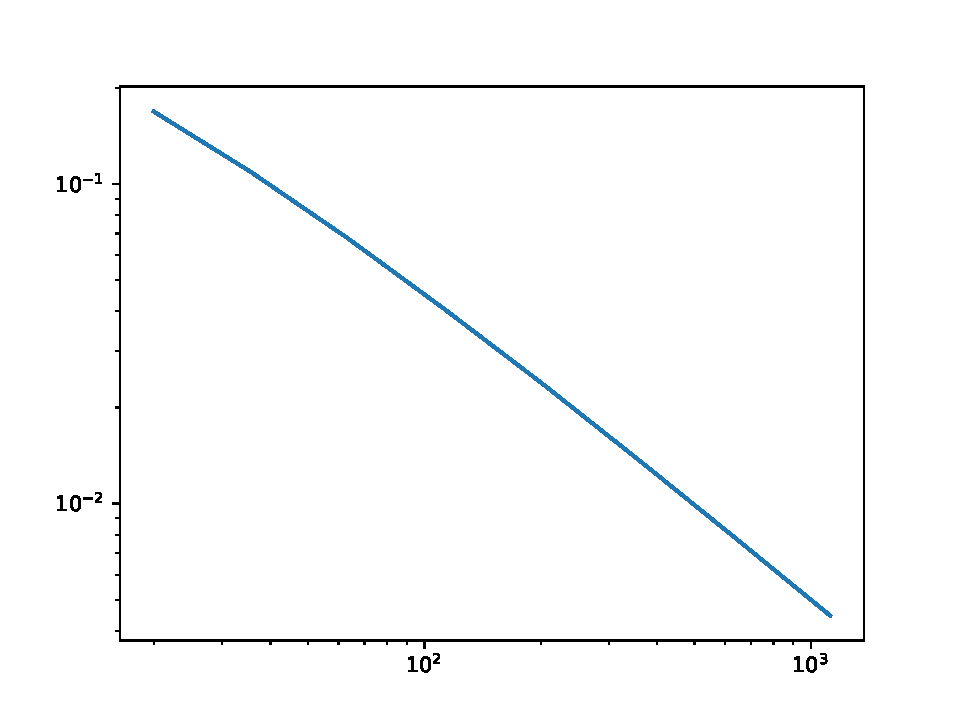
\includegraphics[width=0.75\textwidth]{code/advect_conv.pdf}
    \caption{\label{fig:advect_conv}}
\end{figure}



\subsection{Elliptic Problems}

For elliptic problems, the speed of the propagation is infinite and thus responds instantly to any change the source or boundary conditions. For these sorts of problems, relaxation methods work well, but techniques like multigrid can speed things up. 

Lets consider a problem that arises in astrophysics and electrostatics, the Poisson equation
\be
\nabla^2\Phi = f
\ee
Let's consider the 1-d version first 
\be
\dddx\Phi = f
\ee
with boundary conditions $\Phi(0) = \Phi(1) = 0$.  If we pick $f=\sin(x)$, then we have an analytic solution $\Phi = -\sin(x) +x\sin(1)$.  Given this, how can we solve for this numerically.  

Fortunately, this is an ODE and so the first technique that we will try is using one of our ODE integrators -- say rk2.  Now if we use rk2, we start our and $x=0$ and integrate to $x=1$.  Since $\Phi(x=0) = 0$, we have one initial condition already, but we will need another initial condition for $\Phi'(x=0)$.  We can set this to be a free value, say $\alpha$ and vary it until we get the second boundary condition.  

In other works, lets define a function $g(\alpha)$ such that
\be
g(\alpha) = \Phi(x=1;\alpha),
\ee
where $\Phi$ is computed by numerical integration to $x=1$ using $\Phi'(x=0) = \alpha$.  Since we want $g(\alpha) = 0$, this reduces to a root-finding problem for $\alpha$.  So once we define $g(\alpha)$, we can use root finding routines to find the appropriate value of $\alpha$.  For this, we will use a standard python package. This technique is known as shooting as you are essential shooting until you hit a target.  

\lstinputlisting[language=Python]{code/shoot.py}

Shooting doesn't always work especially with stiff equations which are extremely sensitive to initial conditions.  Examples of this in astrophysics include hydrostatic balance for stars.  In this case, we need to try something different.  Lets discretize the equation to be
\be
\frac{\Phi_{i+1} - 2\Phi_i + \Phi_{i-1}}{\Delta x^2} = f_i,
\ee
where we pick $\Phi_0 = \Phi_N = 0$.  We then have a bunch of algebraic equations:
\be
\Phi_i = 0.5\left(\Phi_{i+1} + \Phi_{i-1} - \Delta x^2 f_i\right).
\ee
In principle, we can solve with matrix inversion, but it is easier to solve using relaxation starting with some initial guess $\Phi_i^0$  This can use either 
\begin{enumerate}
    \item Jacobi iteration: $\Phi_i^{k+1} = 0.5\left(\Phi_{i+1}^k + \Phi_{i-1}^k - \Delta x^2 f_i\right).$
    \item Gauss-Seidel iteration: Use the new $k+1$ values as they appear. 
\end{enumerate}
In either case, you need to keep track of the error to ensure that the error goes down below some threshold. 

Lets look at the code here.
\lstinputlisting[language=Python]{code/relax.py}

which yields the following compared to the analytic result:
\begin{figure}
    \centering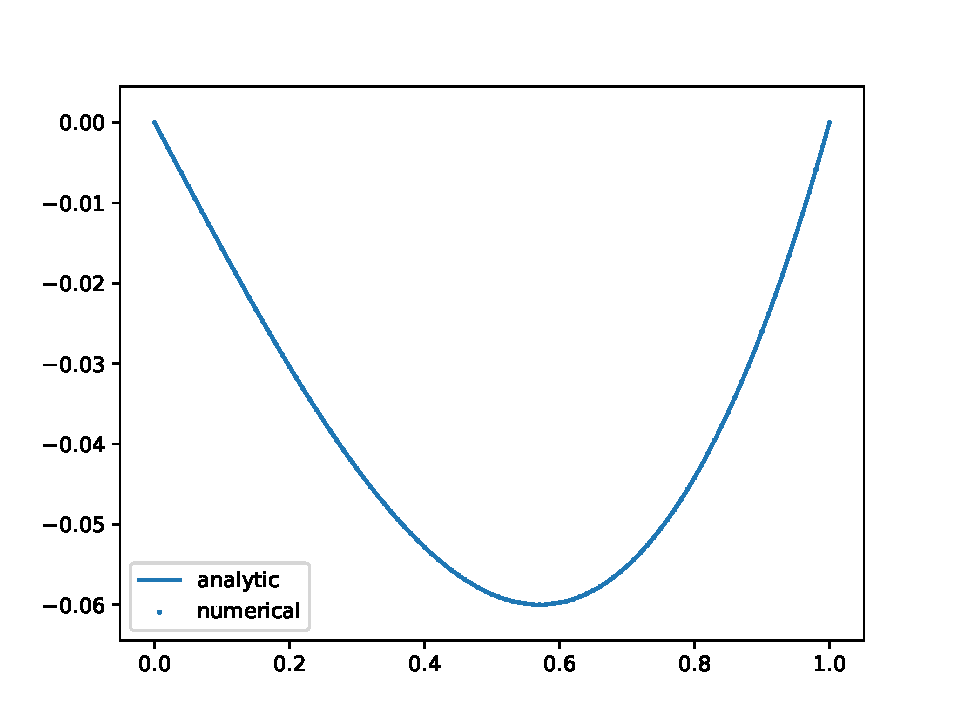
\includegraphics[width=0.75\textwidth]{code/relax.pdf}
    \caption{\label{fig:relax}}
\end{figure}

Running this you can see that theres are quite a few iteration needs to solve this equation. This can be accelerated by coarsening and then refining the grid in a technique known as multigrid. We won't cover this in this as in astrophysics there are other ways to solve this equation (FFTs for instance).

\subsection{Parabolic Problems}

As stated above, the parabolic problem has properties of both the hyperbolic and elliptic problem.  In particular, we will see that it can have very large propagation speeds like the elliptic problem, but can be solve in a flux-conservative way as in the hyperbolic problem.  Lets start with a prototypical problem
\be
\ddt{\Phi} = \dddx{\Phi}\label{eq:diffusion}
\ee
An identification of the flux to the $F = -\partial\Phi/\partial x$ allows us to write this like the flux-conservative equation
\be
\ddt{\Phi} + \ddx{F} = 0
\ee
If we presume the analytic ansatz
\be
\Phi(t,x) = \frac{\exp{-x^2/4t}}{t^{1/2}} + \Phi_0,
\ee
we see that it solve the diffusion equation (\ref{eq:diffusion}).  Lets try to solve this problem numerically.  Lets use a standard centered expression for the second derivative in Space
\be
\frac{\Phi^{n+1}_i - \Phi^n_i}{\Delta t} = \frac{\Phi^n_{i+1} - 2\Phi^n_i + \Phi^n_{i-1}}{\Delta x^2}
\ee
We can examine its stability in space with a single Fourier mode $\Phi_i^n = A^n\exp(-i2\pi x_i/L)$.  This gives
\be
\left|\frac{A^{n+1}}{A^n}\right| = \left|1 + 2\frac{\Delta t}{\Delta x^2}\left(\cos(2\pi\Delta x/L)-1\right)\right| < 1
\ee
which implies that $\Delta t \propto \Delta x^2/2$, e.g., the equivalent ``Courant'' number is $\alpha_{\rm CFL} = 2\Delta t/\Delta x^2$  So the timestep rapidly comes down as $\Delta x$ (higher resolution) shrinks.  

We can numerically solve this once we specific the boundary conditions over a finite domain.  However, we will note that the analytic solution spreads from $x=(-\infty,\infty)$.  However, if we put the boundaries far enough away, it will not ``pollute'' the solution too much in the region of interest.  Here the fact that the timescale goes like $t\sim L^2$ helps. 

Now lets examine the code in detail:

\lstinputlisting[language=Python]{code/parabolic.py}





